


\documentclass[aspectratio=169, 12pt]{beamer}

%%%%%%%%%%%%
% Packages %
%%%%%%%%%%%%

\usepackage{ctex}
\usepackage[english]{babel}
\usepackage{packages/sleek}
\usepackage{packages/tweaks}
\usepackage{calligra} % thanks pakeage
\usepackage{graphicx}

%%%%%%%%%%%%%%%%
% Bibliography %
%%%%%%%%%%%%%%%%

\addbibresource{./resources/bib/references.bib}

%%%%%%%%%%%%%%
% Title-page %
%%%%%%%%%%%%%%


\title{公共经济学}
\subtitle{Public Economics}
\author[LIU ShHUAI]{刘 {  } 帅}
\institute{山西师范大学 {  } 经济与管理学院}
\date{\today}
\titlelogo{./resources/pdf/logo.png}
\framelogo{./resources/pdf/logo.png}

%%%%%%%%%%%%
% Document %
%%%%%%%%%%%%

\begin{document}

\maketitle

\begin{frame}[standout]
    第三章\par
    \addtolength{\parskip}{.4em}
    公共部门规模的衡量
\end{frame}

\begin{frame}[plain]
    \frametitle{重点问题}
    \begin{itemize}
        \item \textbf{政府的主要活动是什么?}
        \item \textbf{政府把钱花在了什么地方?随着时间推移,支出格局发生了怎样的变以及如何进行国际比较?哪些支出是国家层面的,哪些支出是地方层面的?}
        \item \textbf{政府如何为其支出筹资?中央政府和地方政府之间的税收来源有何不同?随着时间推移它们发生了怎样的变化?}
    \end{itemize}
\end{frame}

\begin{frame}[plain]
    % \begin{multicols}{1}
    %   \frametitle{Outline}
    %   \tableofcontents[hideallsubsections]
    % \end{multicols}
    \frametitle{Outline}
    \tableofcontents[hideallsubsections]
    % \tableofcontents[currentsection]
\end{frame}

\section{一、什么或者谁是政府}

\begin{frame}[plain]
    \frametitle{什么或者谁是政府}
    政府与私人机构有两个重要的区别。
    \begin{block}{负责人的产生}
        在民主社会里,负责公共机构运转的人是选举产生的,
        或者是由当选者任命的(或由当选者任命的人所任命的)。
        拥有控制地位的人的“合法性”直接或间接地来源于选举程序。
        相反,私人部门负责人或者管理者不需要选举来确定。
    \end{block}
    \begin{block}{强制权力}
        政府具有一定的强制权力,私人机构则没有。
        政府有权强迫你交税。
    \end{block}
\end{frame}

\section{二、政府活动的类型}

\begin{frame}[plain]
    \frametitle{政府活动}
    政府活动主要包括以下五类:
    \begin{itemize}
        \item \textbf{提供法律制度}
        \item \textbf{生产产品和服务}
        \item \textbf{购买产品与服务}
        \item \textbf{干预私人生产}
        \item \textbf{再分配}
    \end{itemize}
\end{frame}

\begin{frame}[plain]
    \frametitle{政府活动}
    \begin{block}{提供法律制度}
        在法律框架内,企业和个人进行经济交往。
    \end{block}
    \begin{block}{生产产品和服务}
        政府直接从事一些生产,比如电力、饮用水、公立教育、公立医疗、电视广播以及金融等。
        \par
        有时公私生产的区别比较模糊。有许多混合生产模式,
        其特点是公私部门合作,如公共产品和服务提供的公私合伙(Public-private partnerships, PPP)
        和私人部门参与(Private sector participation, PSP)。
    \end{block}
    \begin{block}{购买产品与服务}
        政府购买的特征是把钱花费在公众使用的产品和服务上,例如国防、公立学校、公立医疗和交通道路。
    \end{block}
\end{frame}

\begin{frame}[plain]
    \frametitle{政府活动}
    \begin{block}{干预私人生产}
        政府干预私人生产的手段有补贴、税收、政府贷款和管制。
        \begin{itemize}
            \item 补贴与税收,政府以三大方式补贴私人生产:直接给生产者补贴、通过税制间接给企业补贴(税收抵免)以及其他隐性支出(进口课税)。
            \item 政府贷款,一种特殊的补贴是政府提供利率低于市场利率的贷款,形式有低息贷款和贷款担保。
            \item 监管企业,政府监管企业活动,旨在保护工人、消费者和环境,防止反竞争行为,组织歧视。比如我国的金融监管机构包括“一行两会”,即中国人民银行、银保监会和证监会。市场监管总局,生态环境部等。
        \end{itemize}
    \end{block}
\end{frame}

\begin{frame}[plain]
    \frametitle{政府活动}
    \textbf{政府再分配收入}\par
       有两类显性再分配计划:公共援助计划和社会保险计划。
    \begin{block}{公共援助计划}
        中国政府实施了多种公共援助计划,旨在帮助国内的弱势群体和发展中国家的人民。以下是一些主要的公共援助计划:
        \begin{itemize}
        \item 扶贫计划:中国政府实施了大规模的扶贫计划,旨在帮助贫困地区的居民脱贫。这些计划包括提供基本生活保障、医疗保险和教育支持等。

        \item 援外援助:中国政府向其他国家提供援助,帮助他们发展经济和提高民生水平。这些援助项目包括建设基础设施、提供医疗援助和培训人才等。
        \end{itemize}
    \end{block}
\end{frame}

\begin{frame}[plain]
    \frametitle{政府活动}
    \begin{block}{公共援助计划}
        \begin{itemize}
        \item 灾害救助:中国政府在面对自然灾害和紧急情况时,提供灾害救助和紧急援助。这些救助包括提供物资、住房和医疗支持等。

        \item 教育援助:中国政府向其他发展中国家提供教育援助,帮助他们提高教育水平。这些援助项目包括建设学校、提供教育设备和培训教师等。
        \end{itemize}
    \end{block}
\end{frame}

\begin{frame}[plain]
    \frametitle{政府活动}
    \begin{block}{社会保险计划}
        中国的社会保险计划包括以下几个方面:
        \begin{itemize}
            \item 养老保险:养老保险是指由雇主和员工共同缴纳的,为劳动者在退休后提供经济支持的社会保险。在中国,养老保险主要由企业年金、社会保险基金和个人账户三部分构成。
            \item 医疗保险:医疗保险是指为劳动者提供医疗费用报销、住院津贴等服务的社会保险。在中国,医疗保险主要由城镇职工基本医疗保险、城乡居民基本医疗保险和大病保险三部分构成。
            \item 失业保险:失业保险是指为失业人员提供一定时间的生活补贴和职业培训等服务的社会保险。在中国,失业保险主要由企业和个人缴纳。
        \end{itemize}
    \end{block}
\end{frame}

\begin{frame}[plain]
    \frametitle{政府活动}
    \begin{block}{社会保险计划}
        中国的社会保险计划包括以下几个方面:
        \begin{itemize}
            \item 工伤保险:工伤保险是指为在工作中因意外事故受伤或患职业病的劳动者提供医疗和经济补偿的社会保险。在中国,工伤保险由企业缴纳。
            \item 生育保险:生育保险是指为女性劳动者提供生育津贴和生育医疗费用报销等服务的社会保险。在中国,生育保险由企业缴纳。
        \end{itemize}
    \end{block}
\end{frame}

\begin{frame}[plain]
    \frametitle{政府活动}
        政府不仅通过直接的转移支出影响收入分配,而且通过税收制度(劳动所得税收抵免)和其他
        政府计划间接影响收入再分配。\par
    政府还以补贴和配额的形式对收入进行再分配。中国政府通过免费义务教育、助学金等补贴形式,为低收入家庭的孩子提供教育支持,提高他们的受教育机会和未来收入水平。
    \par
    中国城市户口配额制度规定城市人口必须持有城市户口,且户口数量有限,每年只有一定数量的名额用于农民进城落户。这种制度通过限制城市人口和实行配额管理,调节城市人口结构,促进城乡收入再分配。
    \par
    中国政府采购配额制度规定政府采购商品和服务必须优先选用符合条件的小微企业或社会组织,以提高他们的市场竞争力和收入水平。
\end{frame}

\section{三、公共部门规模的度量}

\begin{frame}[plain]
    \frametitle{国家财政收支总额}
    \begin{figure}
        \centering
        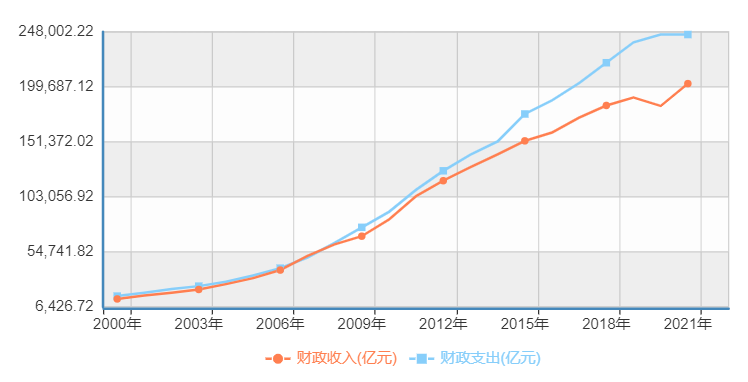
\includegraphics[width=1.0\textwidth]{./resources/figure/finance.png}
    \end{figure}
\end{frame}

\begin{frame}[plain]
    \frametitle{国家财政收支增长率}
    \begin{figure}
        \centering
        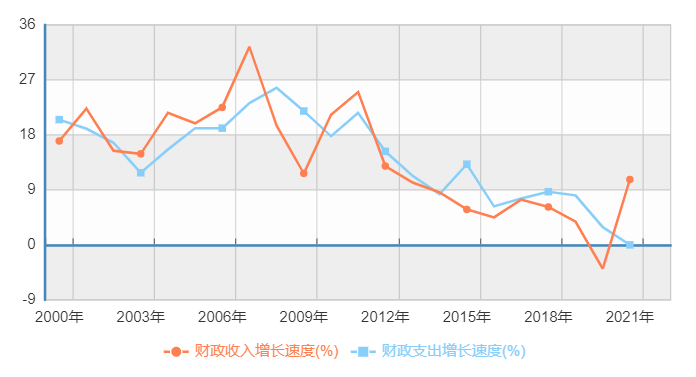
\includegraphics[width=1.0\textwidth]{./resources/figure/finrate.png}
    \end{figure}
\end{frame}

\begin{frame}[plain]
    \frametitle{中央和地方财政支出}
    \begin{figure}
        \centering
        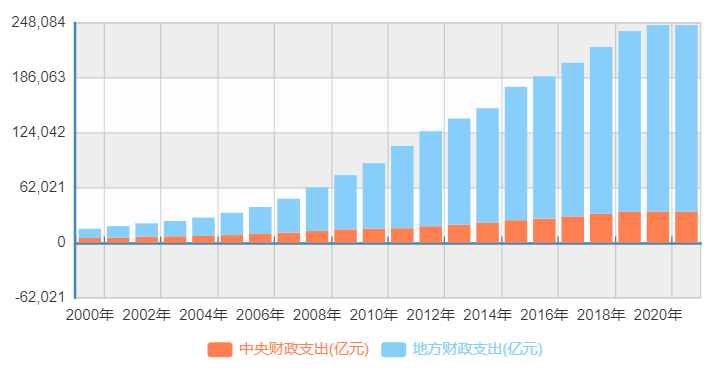
\includegraphics[width=1.0\textwidth]{./resources/figure/spend.png}
    \end{figure}
\end{frame}

\begin{frame}[plain]
    \frametitle{中央和地方财政支出项目}
    \begin{figure}
        \centering
        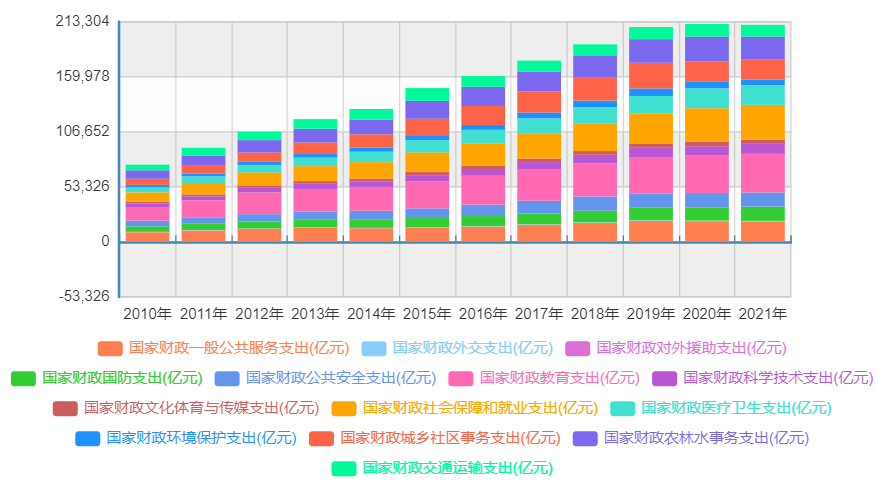
\includegraphics[width=1.0\textwidth]{./resources/figure/spendratio.png}
    \end{figure}
\end{frame}

\begin{frame}[plain]
    \frametitle{中央和地方财政收入}
    \begin{figure}
        \centering
        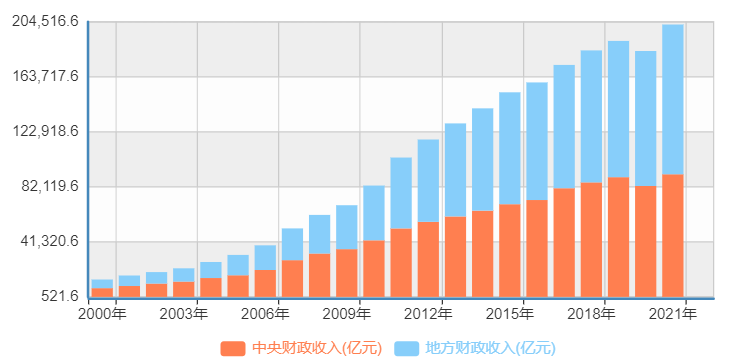
\includegraphics[width=1.0\textwidth]{./resources/figure/income.png}
    \end{figure}
\end{frame}

\begin{frame}[plain]
    \frametitle{中央和地方财政收入项目}
    \begin{figure}
        \centering
        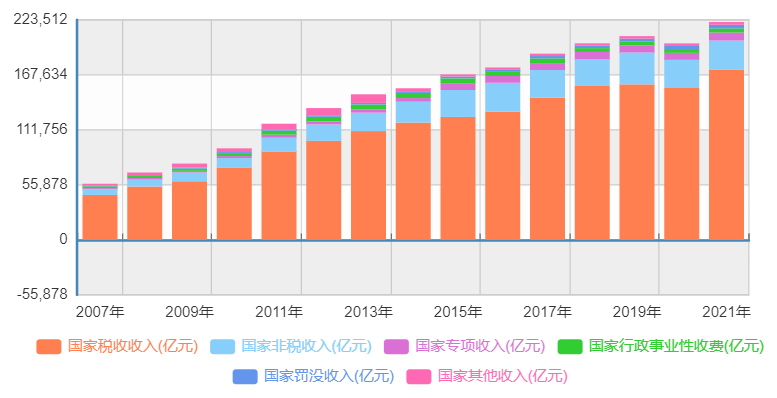
\includegraphics[width=1.0\textwidth]{./resources/figure/incomeratio.png}
    \end{figure}
\end{frame}

\begin{frame}[plain]
    \frametitle{税收项目}
    \begin{figure}
        \centering
        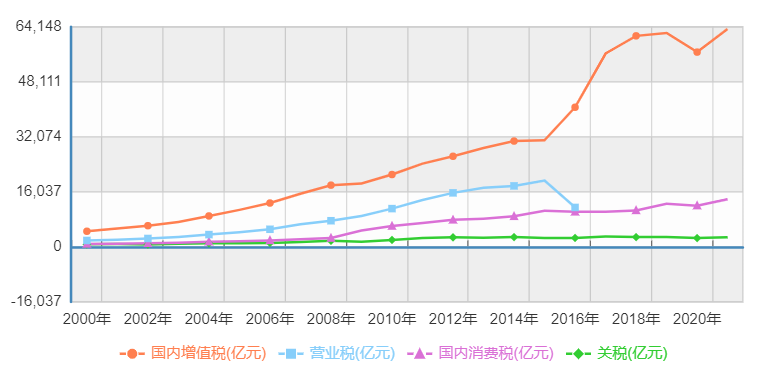
\includegraphics[width=1.0\textwidth]{./resources/figure/tax.png}
    \end{figure}
\end{frame}

\begin{frame}[plain]
    \frametitle{政府债务余额}
    \begin{figure}
        \centering
        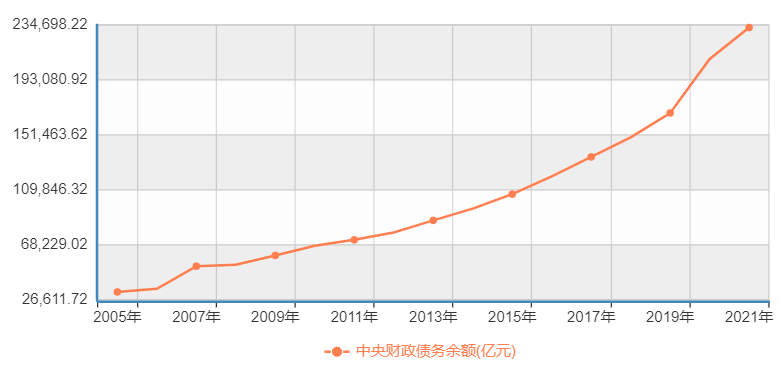
\includegraphics[width=1.0\textwidth]{./resources/figure/debt.png}
    \end{figure}
\end{frame}

\begin{frame}[plain]
    \frametitle{公共部门就业人员}
    \begin{figure}
        \centering
        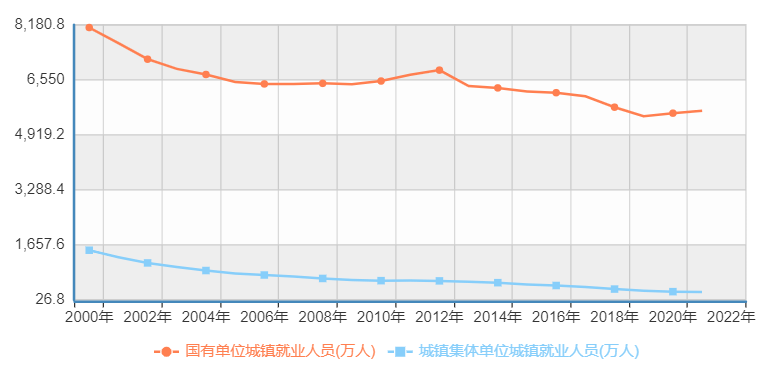
\includegraphics[width=1.0\textwidth]{./resources/figure/employment.png}
    \end{figure}
\end{frame}

% ---------------------------------------------------------------------------
\begin{frame}[standout]
    \begin{center}
        {\Huge\calligra Thanks!}
      \end{center}
\end{frame}
% ---------------------------------------------------------------------------

\end{document}
